% ====================== THE TEXT FILE ===========================

%%    In this file you insert your data -from title to author to references - all the text etc you need for your poster!
%%    You may rename it, but be sure to adjust the name in the setting-file.
%%    If you really have to, you can change the size and color of your text in this file at the beginning of every text frame. The standard size for text is \Large.

% ====================== POSTER COLOR ===========================

%% Choose the color of your poster. You have various possibilities, pick one from the list below and insert it in the \def- brackets, standard for colored background is "ETH5"
%% If you want to have a poster with --- white background ---, please choose a different template for SETTING your tex-file  =>  "Poster-portrait-white.tex" OR "Poster-landscape-white.tex"

\definecolor{ETHBlue}{RGB}{33,92,175}		% blue  
\definecolor{ETHGreen}{RGB}{98,115,19}		% green
\definecolor{ETHPurple}{RGB}{163,7,116}		%  purple for whole page !!
\definecolor{ETHGray}{RGB}{111,111,111}		% gray
\definecolor{ETHRed}{RGB}{183,53,45}		% red
\definecolor{ETHPetrol}{RGB}{0,120,148}		% green/blue 
\definecolor{ETHBronze}{RGB}{142,103,19}	% bronze


\def\linecolor{verylightgray} %%% don't change, necessary for white and colored posters

\graphicspath{{./}{../../../pics-for-poster/}}

\tcbset{
  qbox/.style={
    colback=white,
    colframe=ETHPurple,
    boxrule=0.8pt,
    arc=3pt,
    left=5pt, right=5pt, top=3pt, bottom=3pt,
    fontupper=\small\black
  }
}


% ===========Choose your COLOR here or change it to WHITE  ===========================

 \def\postercolor{ETHPurple} %%% standard for COLORED posters

%\def\postercolor{white} % if your poster has a WHITE background, please define the following parameters as well. Otherwise just command them out
%\def\backgroundcolortitle{ETH3} %%% backgroundcolor of the title box
%\def\backgroundcolorcolor{verylightblue}%%% backgroundcolor of the introduction and conclusion boxes
%\def\backgroundcolorwhite{verylightgray}%%% backgroundcolor for the rest of the boxes




% ======================   POSTER CONTENT ! =====================================

% your first information - will appear as title, author(s), affiliation, partner/sponsors

% ====================== ORGANISATIONAL UNIT ===================
%%your department
\def\department{\linespread{1.1}
\Large Organisational unit,\\
can be spread over 2 lines
}%%% you may have to adjust the position of the text in the setting file, line 102 -> \hspace{}

% ====================== TITLE ===========================
\def\title{
\VERYHuge \white {\bf %%%%
VLMs as Robot Supervisors? \\[10pt]
Benchmarking Multi-View Consistency \\[10pt]
and Failure Mode Detection
}
\\[20pt]}


% ====================== AUTHORS ===========================
%% authors
\def\authors{\LARGE Christian Deubel, Author two$^2$,...}

% ====================== AFFILIATION ===========================

%% affiliations - fill in and extend when necessary the affiliations of your coworkers
\def\firstauthor{$^1$Department of Latex, ETH Zurich, CH}
\def\secondauthor{$^2$Institute for Typesetting, University of Alabama, USA}
\def\thirdauthor{$^3$and so on and on}

\def\affiliations{\LARGE \firstauthor, \secondauthor, \thirdauthor,...}

% ====================== PARTNERS / SPONSORS ===================
%% partners/sponsors
\def\partner{\vspace{5mm}\hspace{0.5cm}\Large Partner/Sponsor:  %your partners/sponsors.
 %You can also include their logos with \{includegraphics}.
}


% ====================== INTRODUCTION ===================
%% 
\def\introtext
{\Large \black
\begin{itemize}
  \item VLMs: promising for robot supervision --- scene interpretation \& semantic feedback, no task-specific training.
  \item \textbf{Multi-view consistency:} does spatial info extracted from different camera angles agree?
  \item \textbf{Failure mode detection:} can a VLM tell when a robotic task went wrong?
  \item Benchmarked across multiple model families --- early signal on VLM strengths/weaknesses as robot supervisors.
\end{itemize}
}%% end text



% ====================== METHOD OVERVIEW ===================
%% 
\def\methodtext
{\large \black
\noindent%
\begin{minipage}[t]{165mm}%
  \centering
  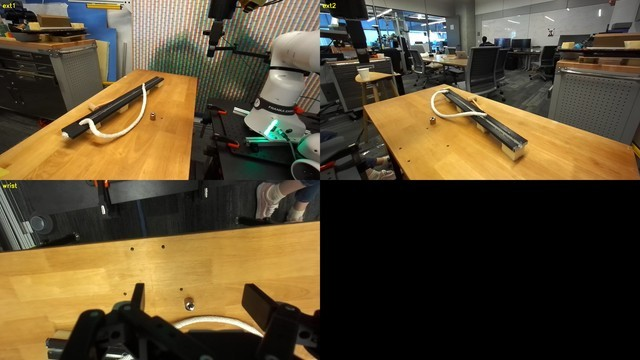
\includegraphics[width=\textwidth]{action_phase_id1_droid_align_the_rope_along_the_middle_of_the_black_object_10648_q14.jpg}\\[4pt]
  \begin{tcolorbox}[qbox]
    \textbf{Action Phase Identification}\\[2pt]
    \textit{Task:} The robot is to align the rope along the middle of the black object.\\[2pt]
    \textbf{Q:} The robot's goal is stated above. Is the robot currently performing the action phase \textit{``gripper moves toward the rope''}?
  \end{tcolorbox}
\end{minipage}\hfill%
\begin{minipage}[t]{165mm}%
  \centering
  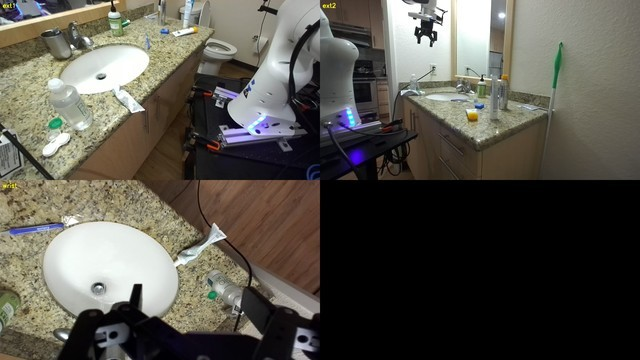
\includegraphics[width=\textwidth]{action_phase_id700_droid_close_the_tap_and_then_remove_the_shaving_stick_from_the_metal_cup_and_put_it_on_the_right_side_of_the_sink_counter_2069_q3.jpg}\\[4pt]
  \begin{tcolorbox}[qbox]
    \textbf{Task Success}\\[2pt]
    \textit{Task:} The robot is to close the tap and then remove the shaving stick from the metal cup and place it on the right side of the sink counter.\\[2pt]
    \textbf{Q:} Did the robot successfully complete the overall task?
  \end{tcolorbox}
\end{minipage}

\vspace{14pt}
\noindent%
\begin{minipage}[t]{165mm}%
  \centering
  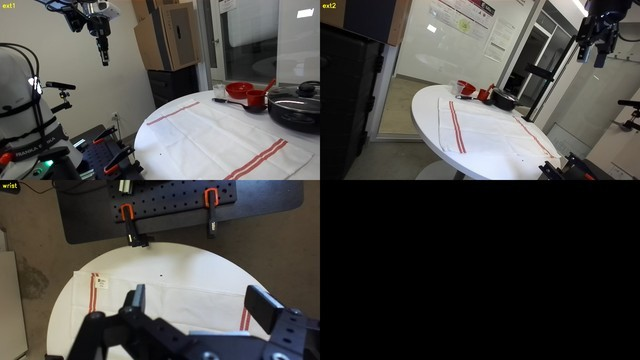
\includegraphics[width=\textwidth]{action_phase_id524_droid_scrunch_up_the_towel_on_the_table_3843_q10.jpg}\\[3pt]
  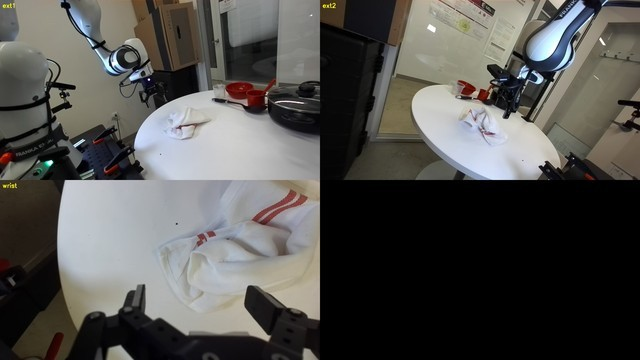
\includegraphics[width=\textwidth]{action_phase_id524_droid_scrunch_up_the_towel_on_the_table_3843_q15.jpg}\\[4pt]
  \begin{tcolorbox}[qbox]
    \textbf{Progress Detection}\\[2pt]
    \textit{Task:} The robot is to scrunch up the towel on the table.\\[2pt]
    \textbf{Q:} The two images were taken during task execution. Did the robot make progress toward completing the goal from Image\,1 to Image\,2?
  \end{tcolorbox}
\end{minipage}\hfill%
\begin{minipage}[t]{165mm}%
  \centering
  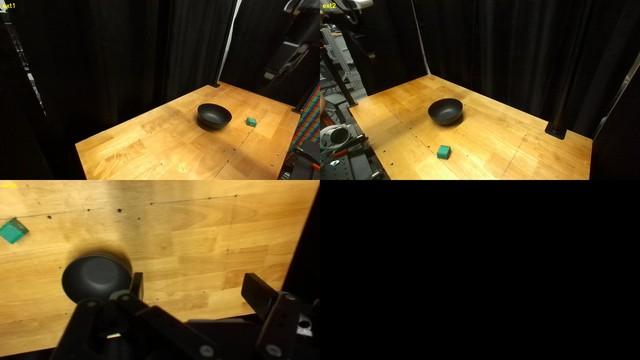
\includegraphics[width=\textwidth]{action_phase_id355_droid_put_the_green_object_inside_the_bowl_2798_q13.jpg}\\[4pt]
  \begin{tcolorbox}[qbox]
    \textbf{Task Success (Adversarial)}\\[2pt]
    \textit{Task:} The robot is to organize all the containers on the white plate.\\[2pt]
    \textbf{Q:} Did the robot successfully complete the overall task? Note: the shown image may depict an unrelated scene.
  \end{tcolorbox}
\end{minipage}
} %% end text


% ====================== MATERIALS ===================
%% 
\def\materialstext
{\Large \black
}%% end text


% ====================== RESULTS / DISCUSSION ===================
%% 
\def\resultstext
{\large \black

\begin{center}
{\large
\begin{tabular}{l|cccc}
\hline
\textbf{Model} & \textbf{Act.Phase} & \textbf{Phase Succ.} & \textbf{Progress} & \textbf{Task Succ.} \\
\hline
Gemma4-31B    & 46.1          & \textbf{46.2} & \textbf{45.2} & 58.8 \\
Gemma4-E4B    & 41.4          & 30.0          & 38.4          & 45.7 \\
Gemma4-E2B    & 31.7          & 24.6          & 35.0          & 37.4 \\
Qwen3-32B     & \textbf{48.0} & 42.6          & 40.9          & 72.2 \\
Qwen3-8B      & 43.5          & 39.5          & 40.2          & 70.9 \\
Qwen3-4B      & 44.8          & 35.6          & 39.1          & \textbf{72.6} \\
InternVL3-14B & 43.8          & 43.8          & 41.7          & 56.2 \\
\hline
Random (uniform) & 33.3 & 25.0 & 33.3 & 33.3 \\
\hline
\multicolumn{5}{l}{\scriptsize All values in \%.}
\end{tabular}
}
\end{center}

% ---- Data sources for table above (action phase, by_task accuracy from summary.json) ----
% Gemma4-31B    : outputs/slurm93218_action_phase_gemma4-31b_default_done/summary.json
% Gemma4-E4B    : outputs/slurm92952_action_phase_gemma4-e4b_default_done/summary.json
% Gemma4-E2B    : outputs/2026-05-31_14-48-00_action_phase_gemma4-e2b_default_done/summary.json
% Qwen3-32B     : outputs/slurm98014_action_phase_qwen3-32b_default/summary.json
% Qwen3-8B      : outputs/2026-05-31_14-44-51_action_phase_qwen3-8b_default_done/summary.json
% Qwen3-4B      : outputs/slurm93661_action_phase_qwen3-4b_default_done/summary.json
% InternVL3-14B : outputs/slurm97555_action_phase_internvl3-14b_default/summary.json
% Column mapping (from "by_task" field): Act.Phase=action_phase_id, Phase Succ.=phase_success,
% Progress=progress, Task Succ.=task_success. "Random (uniform)" row kept from previous
% table version (legacy 1/3 baseline, not recomputed).

\vspace{6pt}

\begin{itemize}
  \item \textbf{Marginal gains over random.} 38.6\,\% overall vs.\ 33.3\,\% random, below 39.6\,\% yes/no baseline.
  \item \textbf{Scene difficulty varies widely.} Gemma4-31B: 34.7--65.3\,\% across 47 scenes (31\,pp spread).
  \item \textbf{Clear, uncluttered scenes work best.} Distinct objects + high contrast $\rightarrow$ highest accuracy.
\end{itemize}

\vspace{14pt}

\noindent\textbf{Multi-view Cross-Camera Consistency}

\vspace{6pt}

\begin{center}
{\large
\begin{tabular}{l|@{\hskip 14pt}ccc}
\hline
\textbf{Model} & \textbf{TL$\leftrightarrow$TR} & \textbf{$\geq$1\,Top$\leftrightarrow$W} & \textbf{All\,3\,Views} \\
\hline
Gemma4-31B      & \textbf{75.9} & 78.9          & \textbf{58.2} \\
Gemma4-E4B      & 61.2          & 71.0          & 45.2 \\
Gemma4-E2B      & 48.3          & 63.7          & 27.9 \\
Qwen3-32B       & 68.4          & 72.1          & 49.2 \\
Qwen3-8B        & 74.8          & \textbf{81.6} & 59.0 \\
Qwen3-4B        & 70.2          & 73.9          & 51.0 \\
InternVL3-14B   & 73.7          & 78.7          & 56.1 \\
\hline
Random (binary) & 50.0 & 75.0 & 25.0 \\
\hline
\multicolumn{4}{l}{\scriptsize All values in \%. TL$\leftrightarrow$TR: top-left agrees with top-right. $\geq$1\,Top$\leftrightarrow$W: at least one top view agrees with wrist. All\,3: all views agree.}\\
\end{tabular}
}
\end{center}

% ---- Data sources for table above (multiview cross-view consistency, "overall" from summary_multiview.json) ----
% Gemma4-31B    : outputs/slurm97655_multiview_gemma4-31b_default_done/summary_multiview.json
% Gemma4-E4B    : outputs/slurm97553_multiview_gemma4-e4b_default_done/summary_multiview.json
% Gemma4-E2B    : outputs/slurm97657_multiview_gemma4-e2b_default_done/summary_multiview.json
% Qwen3-32B     : outputs/slurm98266_multiview_qwen3-32b_default/summary_multiview.json
% Qwen3-8B      : outputs/slurm97947_multiview_qwen3-8b_default/summary_multiview.json
%   *** WARNING: this run is INCOMPLETE -- only 4484/6902 result rows (899/1367 source
%   groups, ~66%) were produced before the job stopped. Numbers will likely change once
%   the run is completed/restarted. ***
% Qwen3-4B      : outputs/slurm97946_multiview_qwen3-4b_default_done/summary_multiview.json
% InternVL3-14B : outputs/slurm97561_multiview_internvl3-14b_default_done/summary_multiview.json
% Column mapping: TL<->TR=tops_agree, >=1 Top<->W=one_top_wrist, All 3 Views=all_agree.
% "Random (binary)" row kept from previous table version (not recomputed).

\vspace{6pt}

\begin{itemize}
  \item \textbf{Clean, contrastive backgrounds help most.} Distinct objects + high contrast $\rightarrow$ best multi-view agreement.
  \item \textbf{Scale helps both tasks.} Larger models improve on multi-view consistency \emph{and} failure detection.
  \item \textbf{Scale isn't enough.} Even on clean scenes, larger models still struggle with multi-view consistency and failure detection.
\end{itemize}

\vspace{14pt}
\noindent%
\begin{minipage}[t]{165mm}%
  \centering
  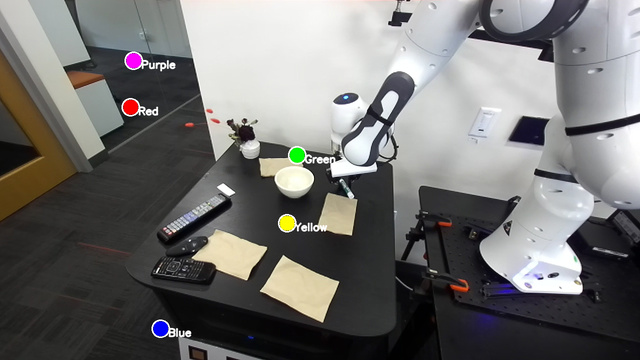
\includegraphics[width=\textwidth]{action_phase_droid_put_the_green_marker_in_the_white_bowl_15148_q10.jpg}\\[4pt]
  \begin{tcolorbox}[qbox]
    \textbf{Easy scene} --- distinct objects, clear spatial reference points, unambiguous task state.
  \end{tcolorbox}
\end{minipage}\hfill%
\begin{minipage}[t]{165mm}%
  \centering
  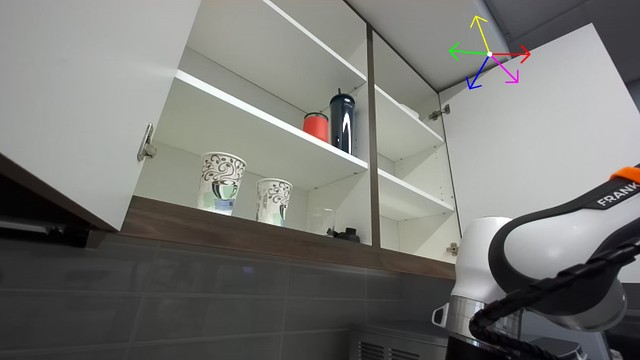
\includegraphics[width=\textwidth]{action_phase_droid_stack_the_two_paper_cups_7914_q10.jpg}\\[4pt]
  \begin{tcolorbox}[qbox]
    \textbf{Difficult scene} --- unusual camera angle, visually similar objects, subtle task state changes.
  \end{tcolorbox}
\end{minipage}

}%% end text


% ====================== CONCLUSION ===================
%% 
\def\conclusiontext
{\Large \black
\begin{itemize}
  \item \textbf{CoT hurts, but reveals reasoning.} Task success drops to 20.9\,\% (below random) --- models describe scenes correctly but draw false conclusions.
  \item \textbf{Scale wins without fine-tuning.} Gemma4-31B leads (47.5\,\%); smaller variants trail by 10--17\,pp.
  \item \textbf{Not built for robot scene understanding.} Strong on object detection/position; weak on \textit{object state} (deformation, orientation, contact) --- rare in web-scale training data.
  \item \textbf{Limitations.} Manual annotation limits scale --- next: automated pipelines + fine-tuning on robotic data.
\end{itemize}
}%% end text



% ====================== REFERENCES ===================
%%
%%% you can use either your normal bib-file, insert file name
\def\bibfile{Poster-content}

%%% or you manually insert your references. In this case make sure to delete the \cite-entries in the dummy text.

\def\bibliotext
{\normalsize \black 
\begin{enumerate}
\item Lorem ipsum dolor sit amet, consectetuer adipiscing elit. Aenean commodo ligula eget dolor. 
\item Cum sociis natoque penatibus et magnis dis parturient montes, nascetur ridiculus mus. 
\end{enumerate}
}%% end text
